% Created 2020-08-07 Fri 16:35
% Intended LaTeX compiler: pdflatex
\documentclass[a4paper,11pt]{article}
\usepackage[utf8]{inputenc}
\usepackage[T1]{fontenc}
\usepackage{graphicx}
\usepackage{grffile}
\usepackage{longtable}
\usepackage{wrapfig}
\usepackage{rotating}
\usepackage[normalem]{ulem}
\usepackage{amsmath}
\usepackage{textcomp}
\usepackage{amssymb}
\usepackage{capt-of}
\usepackage{hyperref}
\author{Tigany Zarrouk}
\date{\today}
\title{Multi-scale investigation of dislocation mediated carbon migration in iron}
\hypersetup{
 pdfauthor={Tigany Zarrouk},
 pdftitle={Multi-scale investigation of dislocation mediated carbon migration in iron},
 pdfkeywords={},
 pdfsubject={},
 pdfcreator={Emacs 26.3 (Org mode 9.1.9)}, 
 pdflang={English}}
\begin{document}

\maketitle
\tableofcontents

\begin{abstract}

We investigate the validity of a dislocation-assisted carbon migration
mechanism underpinning the formation of dark etching regions in
bearing steels undergoing high-cycle fatigue through use of a
multi-scale approach: from quantum mechanics,
to stochastic simulations. We start from tight binding simulations of
$1/3\langle 111 \rangle$ screw dislocations to obtain the 2-d Peierls
potential and Fe-C binding energies. These become ingredients for a line-tension
model of the $1/3\langle 111 \rangle$ screw dislocation to obtain the kink-pair formation
energy as a function of stress and carbon concentration. Finally,
3-d kinetic Monte-Carlo simulations of dislocations in an environment
of carbon are used to ascertain which temperature and stress regimes
dislocation-assisted carbon migration is a valid mechanism. 

\end{abstract}


\section{Introduction}
\label{sec:org8d00b84}

Martensitic steels are frequently used in bearings due to their resilience to service conditions,
being subject to high rotational speeds and contact pressures. However, under cyclic loading
exceeding a given contact stress, the microstructure of the steel can decay due to the accumulation
of plasticity. This signals the onset of rolling cycle fatigue (RCF), which increases the risk of
failure from subsurface crack initiation. The microstructural decay corresponds to the observation
of Dark Etching Regions (DERs) as seen in optical microscopy, where the darkness of these regions is due
to the higher reactivity of the phases which compose the DER to the etchant; exacerbated by
the roughness of the DER region.

Carbon within the martensitic matrix at normal operating temperatures has a low diffusivity; as
such it cannot segregate out of the martensite. A plausible mechanism for the degradation of the
martensitic microstructure is a process of carbon migration, driven by dislocation glide,
described as follows [CITATION]. Due to the high dislocation density exhibited in martensite,
carbon segregates to dislocations in Cottrell atmospheres, causing pinning. Strain
generated by cyclic stresses allow dislocations to escape their carbon rich environment. The
dislocations, now free, re-attract carbon, allowing the Cottrell atmosphere to reform,
subsequently re-pinning the dislocations, creating a net carbon flux.

structure of a WEB consisting of a ferrite band and a LC adjacent to it. One can see the DER region is composed of regions of ferrite interspersed in the parent martensite with lenticular carbides bordering the ferrite bands. 
\begin{figure}[htbp]
\centering
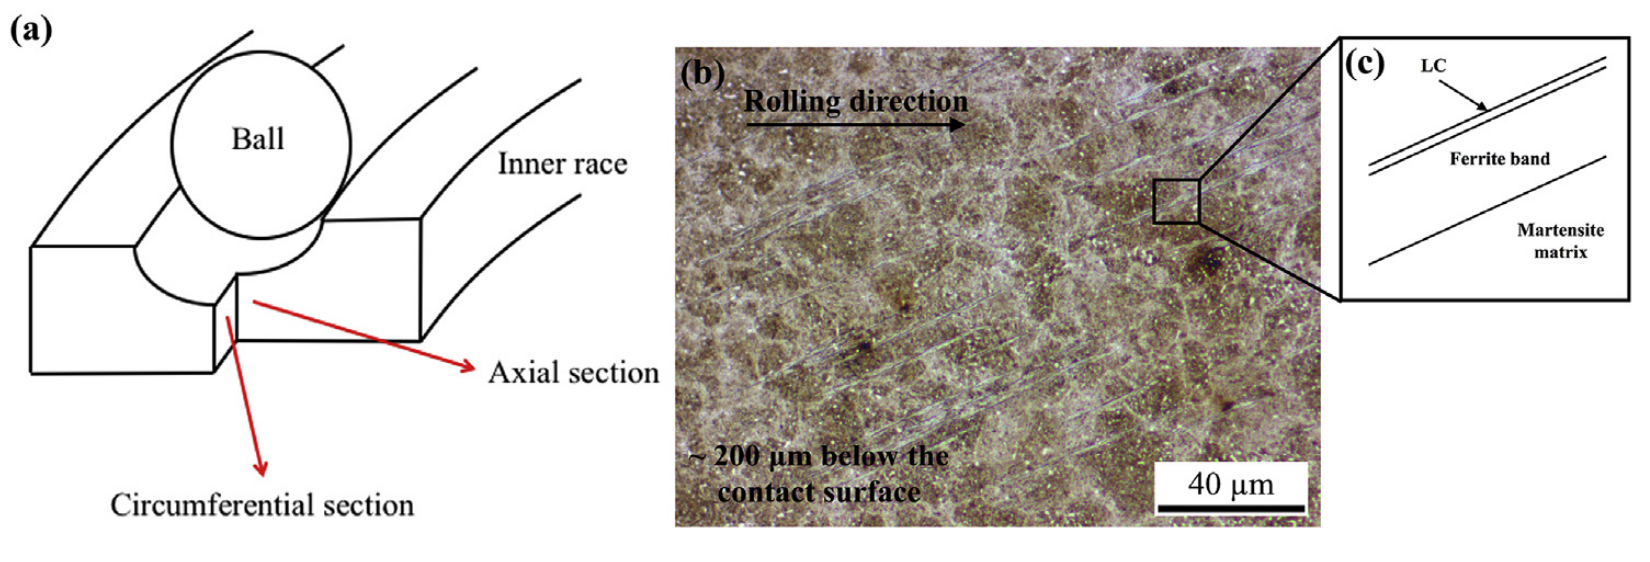
\includegraphics[width=.9\linewidth]{/home/tigany/Documents/docs/Management/Images/der_picture_fu.png}
\caption{\label{fig:org7374b20}
Diagram of where DER occurs and its characteristics, taken from \cite{Fu2017}. (a) Axial and Circumferential sections of a bearing inner ring. (b) Circumferential section of a bearing inner ring under optical microscope, where ferrite bands (white etching bands) are formed at the subsurface with an inclination angle of 30\textdegree{} to the rolling direction. (c) Diagram showing the}
\end{figure}

Through dislocation-assisted carbon migration, martensite transforms to ferrite (microband and
elongated forms). Residual carbides, untouched at the start of DER formation, gradually dissolve
as a result of highly localised plasticity: dislocation rearrangement and pile ups at the
interface draw carbon atoms out. Further RCF progression leads to the formation of low and high
angle ferrite features, White Etching Bands (WEBs), composed from the microband and elongated
ferrite. Carbon migration through dislocation motion allows carbon to move from the martensitic
matrix---and (partially) dissolved residual carbides---to form lenticular carbides between these
ferrite bands. 

However, fundamentals behind DER formation through this process remain contentious. It is not
definitively known where carbon migrates to with the onset of DER formation: where does excess
carbon from the martensitic matrix find itself, when the structure decays to low solubility
(0.02\%) ferrite? It is not known whether carbon atoms inside the martensite are transported
towards the residual transition carbides, \cite{fu17_strain_induc_marten_decay_bearin}, or if they
segregate to the boundaries of ferrite microbands/elongated ferrite.


Fu \emph{et al.} propose that carbon atoms inside the martensite would segregate to
pre-existing/residual carbides, increasing their size
\cite{fu17_strain_induc_marten_decay_bearin}. This theory has been successfully applied to the
growth of lenticular carbides \cite{Fu2017}, however, problems arise with their application to the
growth of residual carbides: if carbides were to form in martensite, they should follow the
Bagaryatskii/Isaichev orientation relationship, but observations suggest a lack of any orientation
relationship \cite{Bhadeshia2018}. Carbides formed within the DER region have an irregular
shape/diffuse boundaries, which are seemingly due to the incomplete \emph{dissolution} of \emph{residual}
carbides, which is at odds with the theory of Fu \emph{et al.} and residual carbide growth.



Probing the fundamental mechanisms behind DER formation experimentally have proven difficult and
inconclusive. Work needs to be done to understand dislocation-carbon interactions, more specifically, how
dislocations can move carbon within the temperature and stress regimes experienced during
operation, and what phenomena occur during dislocation-assisted carbon migration. This is vital to
understanding martensite decay and DER formation. With further knowledge of the fundamental
mechanism behind DER formation, we can surpress dislocation motion in the martensitic
matrix, mitigating failure by RCF.

To shed light on the fundamental mechanism underpinning DER
formation---dislocation-assisted carbon migration---a multi-scale modelling approach can be
used. Atomistics can provide information of the 2d Peierls energy landscape which dislocations are
subject to in iron; and how this landscape is modified by the binding of carbon to
dislocations. This data can be used in a line tension model of a dislocation, to determine the
kink-pair nucleation energies of dislocations as a function of carbon content and stress. Finally,
one can use a kinetic Monte Carlo model of dislocation glide, by thermally activated kink-pair
nucleation, in an environment of carbon. From this last stage of coarse-graining, one can
determine in which regimes of temperature, stress and carbon concentration, dislocation-assisted
carbon migration becomes a feasible mechanism behind DER formation, with predictions of
dislocation velocity and where carbon moves to as dislocations glide. In this report, we will focus
on the atomistic portion of this project, directed at understanding dislocation-carbon interactions at the
atomistic scale in bcc iron, which will feed into the line-tension model of dislocation kink-pair formation.







\section{Computational Method}
\label{sec:org306cf70}

We use the tight-binding model of Paxton and Elsätter \cite{Paxton2013}, which has been
shown to describe the binding energies of carbon complexes in bcc iron, in good agreement with
high-quality Density Functional Theory (DFT) calculations. This model reproduces the
two screw dislocation core structures---the easy and hard \(1/2\langle 111 \rang\) cores---exhibited in bcc
iron, which are crucial to understanding solute-dislocation interactions in bcc iron. Hydrogen and
carbon have been shown to reconstruct these cores into the, usually metastable, hard core from
the easy core \cite{Ventelon2015,itakura13_effec_hydrog_atoms_screw_disloc}. Computationally cheaper models, which
do not incorporate quantum mechanics, such as the EAM, cannot reproduce these behaviours.


To determine the Peierls potential of a \(1/2\langle 111 \rang\) screw dislocation, we followed the procedure detailed in Itakura
\cite{Itakura2012}. Quadrupolar arrays of dislocations were constructed by placing dislocations of
antiparallel \(1/2\langle 111\rangle\) Burgers vectors in an "S" arrangement \cite{Clouet2012}, see
\ref{sarrangementclouet}, with initial displacements determined by the anisotropic elasticity
solutions. These displacements were modified to be periodic, thereby removing artificial stacking
faults which would appear between periodic images after the introduction of the dislocation
dipole. This was achieved by the subraction of a linear error term from the superposition of
displacement fields arising from the dislocations in the simulation cell and its periodic images
\cite{vasilybulatov2006}. To accomodate for the internal stress upon introduction of the
dislocation dipole into a simulation cell, an elastic strain was applied to the cell, resulting
in an additional tilt component added to the cell vectors
\cite{Clouet2012,vasilybulatov2006}. Simulation cells were constructed with different initial core
positions, which were sampled from the triangular region "EHS" (easy, hard and split) core
positions, as detailed in \ref{sampledpositions}. To fix the dislocation positions during relaxation,
the three atoms surrounding the easy core, for each dislocation, were fixed in Z coordinate
during relaxation. Relaxations were carried out until forces on each atom were less than \(1\times10^{-3 }\text{eV}\AA^{-1}\).


\begin{center}
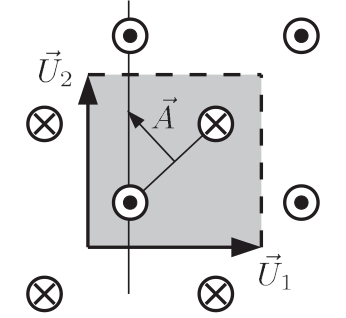
\includegraphics[width=0.5\textwidth]{/home/tigany/Documents/docs/Management/Images/s_arrangement_clouet.png}
\captionof{figure}{\label{fig:orgbb85e15}
Figure of the quadrupolar arrangement used to determine the Peierls potential. \(\vec{U}_1\) and \(\vec{U}_2\) are the periodicity vectors in the X-Y plane. \(\vec{A}\) is the vector defining the cut plane of the dislocation dipole \cite{Clouet2012}.}
\end{center}

\begin{figure}[htbp]
\centering
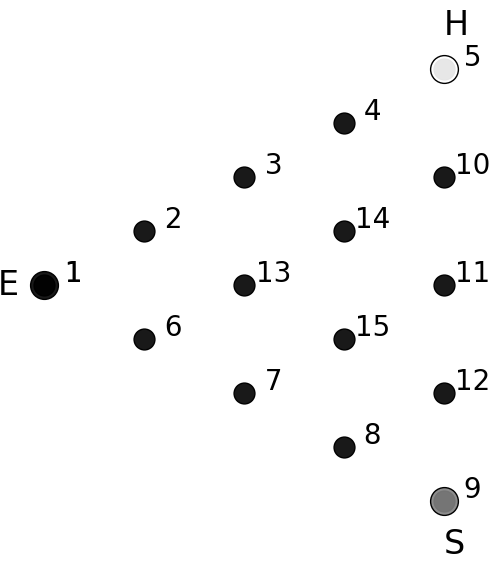
\includegraphics[width=0.45\textwidth]{/home/tigany/Documents/docs/Management/Images/peierls_potential_positions_tbe.png}
\caption{\label{fig:orgd36efd5}
Figure of the sampled positions used to determine the the Peierls potential. "E", "H" and "S" correspond to the easy, hard and split core positions respectively.}
\end{figure}


The interaction energy between the dislocation dipole and periodic images was defined differently
to that of Itakura's. We followed the prescription of Bulatov and Cai \cite{vasilybulatov2006} to
find a regularised interaction energy, which is independent of truncation limit, in contrast to
the formulas quoted in Itakura's papers \cite{Itakura2012}. Details can be found in \ref{sec:Ainteractionenergy}.


The Peierls potential here is defined relative to the energy of the easy core configuration. The
difference in total energies is taken between a relaxed cell, where the dislocation cores are
displaced, from the periodic easy core reference, with a correction term coming from the
difference in interaction energies between the displaced state and the easy core, due to the
difference in dislocation positions. \(\Delta\) henceforth refers to quantities relative to the easy
core configuration, divided by the total number of dislocations in the reference cell. 

\[ \Delta E_{\text{P}} = \Delta E^{\text{tbe}} - \Delta E_{\text{INT}} \]



To determine the binding energy of carbon to dislocations, we used the
cluster method: simulation cells consist of a cylindrical cluster of
atoms, with a single dislocation introduced into the
centre using displacements from the anisotropic elasticity solutions. Each of the clusters
were centred on the easy or hard core positions. The cluster of atoms was
split into two regions: a central region of dynamic atoms with radius \(R_1\),
and an annulus of atoms, between \(R_1\) and \(R_2\), which were fixed to the anisotropic
elasticity solutions. 

Initially, large cells of with \(R_1 = 6\sqrt{2}a_{\text{bcc}}\), and \(R_2 =
   7\sqrt{2}a_{\text{bcc}}\) and depth of single burger's vector, were relaxed
for both the easy and hard cores, which consisted of 522 and 540 atoms
respectively. The three atoms surrounding the core were constrained, to only
relax in \(X-Y\) plane, to stop the core from moving upon relaxation. The
k-point sampling mesh for each of these cells was 1x1x24, with a charge
tolerance for self-consistency of \(1\times10^{-6}\). Atoms were relaxed until the force
on each atom was less than \(1\times10^{-3}\) eV\AA{}\(^{\text{-1}}\).  

From the relaxed cells, a smaller region of 174 atoms, with \(R_1 =
   3\sqrt{2}a_{\text{bcc}}\), and \(R_2 = 4\sqrt{2}a_{\text{bcc}}\), was cut from
the dynamic regions. This smaller cell was extended to a thickness of 3\(b\) in
the \(Z\) direction. Carbon interstitials were inserted into octahedral sites
near the dislocation core, in the middle layer. Exploiting reflection and
rotational symmetry, allows us to use only 10 interstitial
sites to obtain the binding energies of carbon \(\sim2\) b from the core. 

The three atoms surrounding the core in the first and third layers were again
constrained to relax only in the \(X\) and \(Y\) directions. No such constraints
were imposed on the middle layer. 




Following the paper by Itakura
\cite{itakura13_effec_hydrog_atoms_screw_disloc} we calculated the
binding energy of carbon each of the screw dislocation cores. 

The solution energy is given by 
\[ E_s = E_{\text{d + C}} + E_{\text{Perfect}}- E_{\text{d}} - E_{\text{C ref.}}, \]
where \(E_{\text{d + C}}\) is the total energy of a relaxed cluster with a
carbon interstitial and a dislocation, \(E_{\text{d}}\) is the total
energy of a relaxed cluster with a dislocation and \(E_{\text{C
    oct.}}\) is the total energy of relaxed a cluster with a single carbon in
an octahedral site.

The zero-point energy is calculated as in Itakura. After relaxation of the
C-dislocation system, a 3x3 Hessian matrix is constructed by taking the
numerical derivative of forces observed on the carbon atom after
displacement by \(\pm 0.015 \AA\) in each of the \(X\), \(Y\) and \(Z\) directions.
The three atoms surrounding the core on the first and third layers were
again fixed in \(Z\) coordinate. The zero-point energy is
given by

\[ E_z = \frac{1}{2} \sum_{i=1}^3 \frac{h}{2\pi} \sqrt{ k_i /
    m_{\text{C}} },  \]
where \(k_i\) are the eigenvalues of the Hessian and \(m_\text{C}\) is
the mass of carbon. 

The ZPE corrected solution energy is given by 
\[ E^{\text{Z}}_{s} = E_s + \Delta E_z,  \]

where \(\Delta E_z = E_z - E_{z\text{C ref.}}\) and \(E_{z\text{C ref.}} = 202.5 meV\) is the zero-point energy of carbon
situated in an octahedral site in a perfect cluster of the same size. The difference in
zero-point energy was found to be negligible in comparison to the binding energies, as one would
expect from an atom much larger than hydrogen. 



\section{Results}
\label{sec:orga092f71}

\subsection{Peierls Potential}
\label{sec:org5aa6bf7}

        \begin{table}
    \begin{tabular}{c}
	     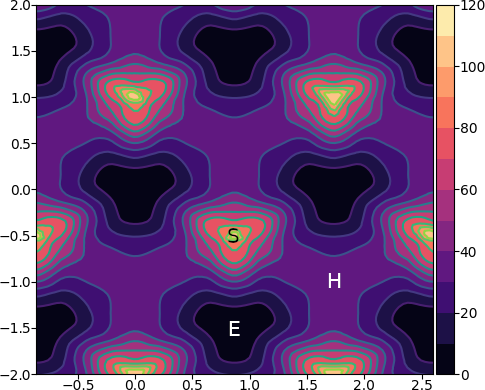
\includegraphics[width=0.8\textwidth]{../Images/itakura_dislocation_energy_landscape_2_labelled.png} \\
             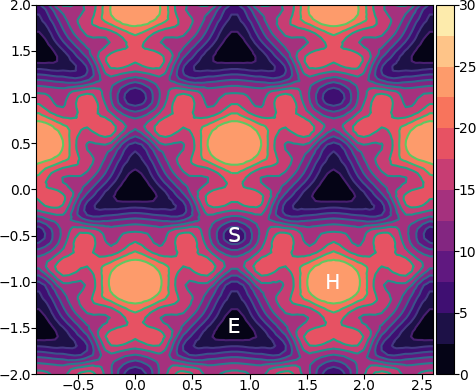
\includegraphics[width=0.8\textwidth]{../Images/tbe_dislocation_energy_landscape_pure_labelled.png}  \\
    \end{tabular}		
\caption{Comparison of 2d Peierls potentials of the $1/2\langle 111\rangle$ screw dislocation between DFT cite:Itakura2012 (top) and tight-binding (bottom). Data was interpolated using cubic splines. Energies are in $meV$, with x and y scales in units of $\sqrt{2} a_{\text{bcc}} = 2\sqrt{2/3}b$. "E", "H" and "S" correspond to easy, hard and split core positions respectively, with the latter also corresponting to atomic positions. The relative energies between the different core positions is smaller in tight-binding compared to DFT. The split core as seen in tight-binding is reminiscent of EAM potentials, where the split core energy is lower than that of the hard core. Some of this discrepancy can be attributed to the difference in interaction energy definitions.}
	\label{fig:peierlspot}
    \end{table}



Comparison of 2d Peierls potentials of the \(1/2\langle 111 \rangle\) screw dislocation between DFT and
tight-binding can be found in \ref{fig:peierlspot}. Data was interpolated using 2d cubic splines. "E", "H" and "S"
correspond to easy, hard and split core positions respectively, with the latter also
corresponding to atomic positions. 
The relative energies between the different core
positions is smaller in tight-binding compared to DFT; most notably, the energies. This is
an artifact in the model, which has been validated in NEB calculations of the \(1/2\langle 111\rangle\)
screw dislocation Peierls barrier: the tight-binding Peierls barrier half that of DFT
\cite{Simpson2019}. The split core as seen in tight-binding is reminiscent of EAM potentials,
where the split core energy is lower than that of the hard core \cite{Itakura2012}. Some of
this discrepancy can be attributed to the to erroneous interaction term included by Itakura,
as detailed above---interaction energies can become arbitrarily high, if not made independent of
truncation limit---but likely, there are effects in DFT which are not encapsulated fully
within tight-binding (or EAM), such as a lack of core electron repulsion or environmental
dependence. 

\begin{center}
\begin{tabular}{rrrrr}
Pos & \(\Delta E_{\text{INT}}\) & \(\Delta E_{\text{tbe}}\) & \(\Delta E_{\text{P}}\) & \(\Delta E_{\text{P}}^{\text{DFT}}\)\\
\hline
1 & 0 & 0 & 0 & 0\\
2 & -0.7 & 7.3 & 7.9 & 3.2\\
3 & -1.4 & 16.0 & 17.4 & 19.2\\
4 & -2.0 & 22.2 & 24.2 & 31.1\\
5 & -2.5 & 24.8 & 27.4 & 39.3\\
6 & -3.3 & 3.0 & 6.3 & 11.5\\
7 & -6.5 & 7.1 & 13.6 & 39.9\\
8 & -9.6 & 13.0 & 22.6 & 75.2\\
9 & -12.5 & 5.4 & 17.9 & 108.9\\
10 & -4.8 & 22.1 & 26.9 & 34.8\\
11 & -7.2 & 18.2 & 25.4 & 37.9\\
12 & -9.8 & 14.0 & 23.8 & 60.7\\
13 & -3.8 & 11.5 & 15.3 & 17.6\\
14 & -6.9 & 15.1 & 22.0 & 29.9\\
15 & -4.3 & 18.6 & 22.9 & 39.7\\
\end{tabular}
\end{center}

\subsection{Hard and easy core relaxations}
\label{sec:org2f71f2d}


To validate the cluster simulation method, the excess energy, defined as the difference in energy between
a cell with a dislocation, and a perfect reference cell, was plotted as as function of
\(\text{ln}(R/r_c)\), where \(R = R_2\) of the cluster and \(r_c = b\), is the core radius, as seen in
figure \ref{lnrdep}. In
elasticity theory, this should give a linear dependence where the gradient corresponds to
combinations of elastic constants. This is well reproduced by our model, except at low
\(\text{ln}(R/r_c)\) as expected, where the cell size is not large enough to accommodate for sufficient
relaxation of the dislocation cores. This increases the core energy, which elasticity theory does
not account for.

\begin{figure}[htbp]
\centering
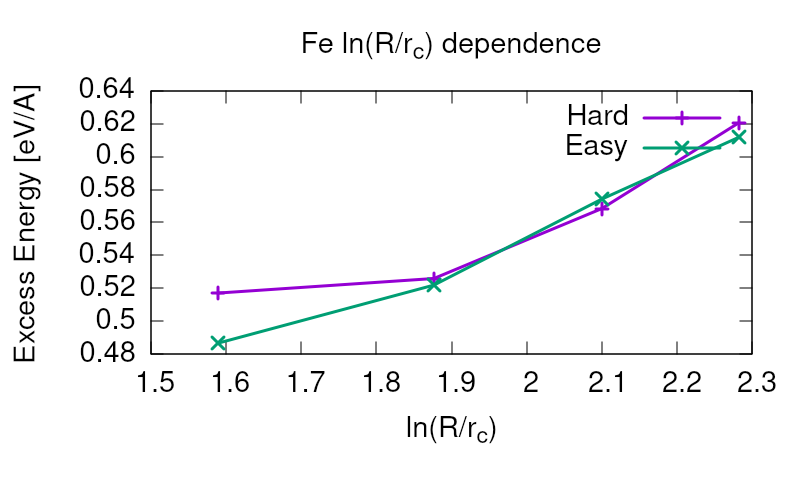
\includegraphics[width=.9\linewidth]{/home/tigany/Documents/docs/Management/Images/img_fe_size_dependence_on_log_of_core_radius.png}
\caption{\label{fig:orgd008941}
Excess energy of dislocation clusters with differing radii for both the easy and hard core configurations. The prediction from elasticity theory is given by the black, dashed line. Deviation of both cores occur when cell size is small, creating an increase in the core energy, which elasticity theory cannot account for.}
\end{figure}




As found in DFT simulations by Ventelon \cite{Ventelon2015}, when a carbon was placed in the
vicinity of a relaxed easy dislocation core---in either of the two nearest, distinguishable,
octahedral sites---a spontaneous reconstruction of the dislocation core occurred: from easy to
hard. Upon reconstruction, the dislocation core moved to a neighbouring triangle, when looking along the \(\langle
   111\rangle\) direction, where the carbon found itself situated in the centre. This will be called a
prismatic site, as in Ventelon's paper. This model successfully
reproduces this behaviour, confirming that both hard and easy dislocation cores must be studied
to fully understand screw dislocation behaviour in bcc iron. 


The core energy difference can be estimated by the difference
between of excess energies between the easy and hard cores in the limit
that \(\text{ln}(\frac{R}{R_0}) \rightarrow 0\). At the smallest
value, one finds that the core energy difference \(\Delta
   E_c^{\text{Easy-Hard}} = 76\) meV/b. This is in agreement with the
results of Itakura \cite{Itakura2012}, of 82 meV/b.



\subsection{Fe-C binding energies}
\label{sec:org997b4e9}

The binding energies, and distribution, of carbon to both the hard and easy cores can be seen in table
\ref{tab:bindingenergies} and figures \ref{easybindingenergydist} and \ref{hardbindingenergydist}. The
distribution of carbon strongly depends on the type of core it finds itself situated near. 

The easy core only significantly modifies the position of the iE1 site, to the E1 site, situated
in the centre of an adjacent triangle. All other sites are unaffected, so there is a one-to-one
correspondence between all \(\text{iE}x\) and \(\text{E}x\) sites. There are carbon basins available
close to the core, but not inside: a pseudo-prismatic site is not favourable.

Carbon favours a prismatic site within the hard core (H1), which has the highest
binding energy of all sites in both cores of 1.29 eV. There are no binding sites apparent in a triangular
annulus (of width \(\sqrt{2}/2 a_{\text{bcc}}\)) surrounding the hard core triangle due to the
destruction/volume reduction of octahedral sites near the hard core. The initial "octahedral"
sites, iH1 and iH2 decay to the H1 site. Similarly, iH3 and iH4 decay to the H2 site, with iH9
and iH10 decaying to a H7 site. Relations between each of the sites is given in table
\ref{decayrelations}.

\begin{table}[htbp]
\caption{\label{tab:org8d275ce}
Decay relations between the initial and final sites upon relaxation of carbon intersitials around the hard core.}
\centering
\begin{tabular}{ll}
Initial & Final\\
\hline
iH1, iH2 & H1\\
iH3, iH4 & H2\\
iH5 & H3\\
iH6 & H4\\
iH7 & H5\\
iH8 & H6\\
iH9, iH10 & H7\\
\end{tabular}
\end{table}


Note that interactions between carbon atoms around the core are not taken into account here:
figures \ref{easybindingenergydist} and \ref{hardbindingenergydist} are purely diagrammatic and not
what one expects the true distribution of carbon would be around a screw dislocation. Carbon is strongly
repulsive at first nearest-neighbour distances, which would modify each of these
distributions. Further work is necessary to elucidate the equilibrium distribution at different
carbon concentrations. 


\begin{table}	
    \begin{tabular}{l}
 	          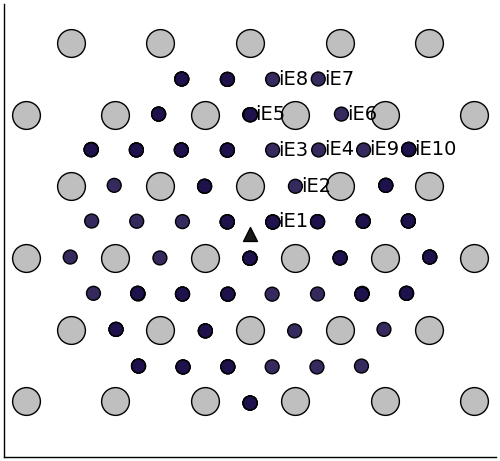
\includegraphics[width=0.7\textwidth]{../Images/easy_core_fe_C_initial_positioning.png}  \\
 	          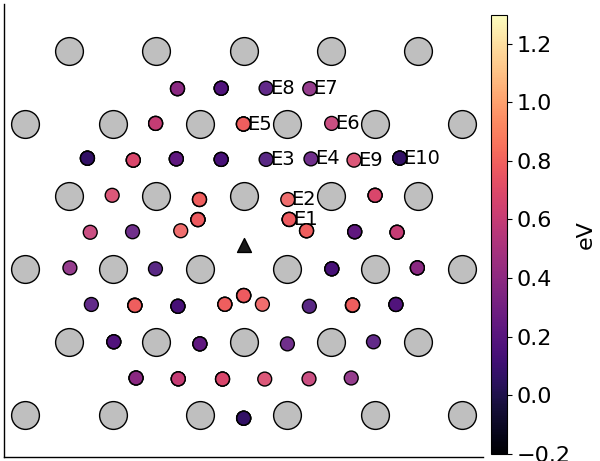
\includegraphics[width=0.85\textwidth]{../Images/easy_core_fe_C_positioning_energies_e10_label.png}  \\

     	     \end{tabular}		
\caption{ Initial and final positions and binding energies (eV) of carbon around the easy core. Binding energies are not shown for the initial positions. Top: initial positions before relaxation. Bottom: final positions and binding energies after relaxation. The core was constrained by fixing the top and bottom three atoms surrounding each of the cores. As shown by Ventelon \cite{Ventelon2015}, the first and second closest octahedral sites to the hard core decay to a prismatic position inside the hard core. }
\label{easybindingenergydist}
   \end{table}


\begin{table}	
    \begin{tabular}{l}
 	          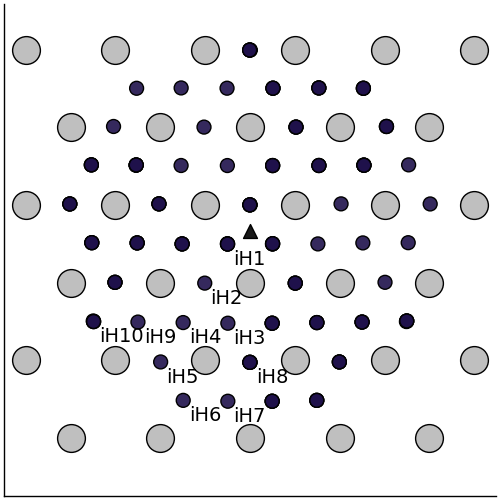
\includegraphics[width=0.7\textwidth]{../Images/hard_core_fe_C_initial_positioning.png}  \\
 	          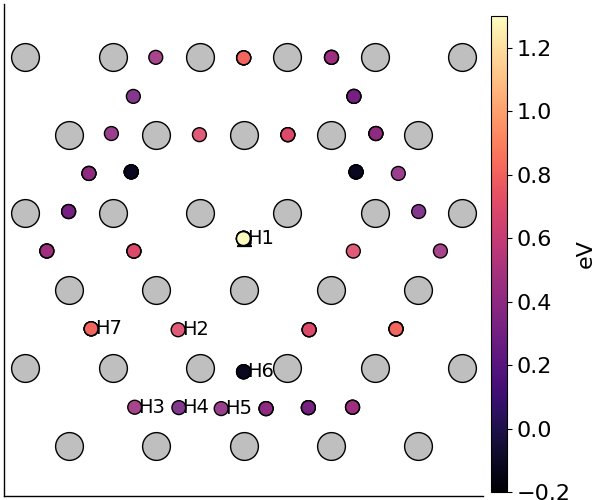
\includegraphics[width=0.85\textwidth]{../Images/hard_core_fe_C_positioning_energies_h7_label.png}  \\

     	     \end{tabular}		
\caption{ Final positions and binding energies (eV) of carbon around the hard core. Top: initial positions before relaxation. Bottom: positions after relaxation. The core was constrained by fixing the top and bottom three atoms surrounding each of the cores. As shown by Ventelon \cite{Ventelon2015}, the first and second closest octahedral sites to the hard core decay to a prismatic position inside the hard core. }
\label{hardbindingenergydist}
   \end{table}




\begin{table*}
    \begin{tabular}{cccccc}
    \hline
Site Type & distance from core [b] & $E^{z}$ [eV] & $\Delta E^{z}$ [eV] & $E_b$ [eV] & $E_b^{z}$ [eV]  \\ 
     \hline
% 00        &                    --  &   0.203      &               0.000 &             &         --     \\
%           &                        &              &                     &             &                \\\hline
E1        &                   0.57 &   0.185      & 	     -0.018 &       0.793 &          0.775 \\
E2        &                   0.70 &   0.202      & 	     -0.001 &       0.793 &          0.793 \\
E3        &                   0.99 &   0.205      & 	      0.002 &       0.137 &          0.139 \\
E4        &                   1.21 &   0.208      & 	      0.005 &       0.229 &          0.234 \\
E5        &                   1.36 &   0.210      & 	      0.008 &       0.784 &          0.791 \\
E6        &                   1.66 &   0.209      & 	      0.007 &       0.597 &          0.603 \\
E7        &                   1.89 &   0.206      & 	      0.003 &       0.385 &          0.388 \\
E8        &                   1.77 &   0.203      & 	      0.000 &       0.177 &          0.178 \\
E9        &                   1.52 &   0.201      & 	      0.000 &       0.683 &          0.683 \\
E10       &                   1.95 &   0.202      & 	      0.000 &       0.067 &          0.067 \\ \hline
H1        &                   0.00 &   0.196      & 	     -0.006 &       1.298 &          1.291 \\
H2        &                   1.19 &   0.210      & 	      0.007 &       0.691 &          0.698 \\
H3        &                   2.12 &   0.209      & 	      0.007 &       0.461 &          0.467 \\
H4        &                   1.91 &   0.207      & 	      0.005 &       0.311 &          0.316 \\
H5        &                   1.80 &   0.208      & 	      0.006 &       0.403 &          0.409 \\
H6        &                   1.40 &   0.207      & 	      0.005 &      -0.119 &         -0.114 \\
H7        &                   1.35 &   0.206      & 	      0.006 &       0.825 &          0.819 \\

    \end{tabular}		
    \caption{Table of energies leading to the zero-point energy corrected binding energy using the cluster method for simulation of dislocation-carbon interactions. }
    \label{tab:bindingenergies}
\end{table*}

These binding energies agree well with experiment and previous calculations.  Kamber \emph\{et
al.\} found a maximum binding energy of 0.5 eV. Cochardt found a value of 0.71 eV, which is
within 0.1eV of the largest binding energy for the easy core.

EAM calculations by Clouet \cite{Clouet2008,Becquart2007} found a maximum binding energy of 0.41 eV by
calculating the elastic dipole tensor within Eshelby theory. Hanlumyuang \emph{et al.}
\cite{Hanlumyuang2010}, similarly conducted DFT and EAM calculations for the interaction energy
12\AA{} from the core, and their calculations agreed with the continuum limit of Eshelby theory with
a binding energy of 0.2 eV.

In work by Ventelon \cite{Ventelon2015}, the interaction energy of a carbon in a hard
core prism configuration was found to be 0.79 eV for a thickness in the \(Z\) direction of 3\(b\) (0.73eV for \(6b\))---in the
convention that a positive binding energy indicates attraction. This is significantly lower than
the 1.29eV interaction energy of tight-binding. 

This discrepancy can be partially explained by the fact that the cells have not been allowed to
relax with all degrees of freedom, as in the Ventelon results: the three atoms around the screw
core are fixed in Z to fix the dislocation core position. A larger source of error is likely
to do with the fitting of the tight-binding model itself. The Peierls barrier of this s-d model
of iron, necessary for Fe-C interactions, has been show to be half that found in DFT, or the
canonical d model \cite{Simpson2019}, but the solution energies for Fe-C defect complexes are well
described. This implies there is insufficient repulsion between Fe-Fe species, upon deformation,
leading to a higher Fe-C binding energy from tight-binding, compared to DFT.


Analysing these results, one can predict the equilibrium carbon concentration of a given carbon
binding site, assuming carbon atoms around the core are sufficiently spaced such that intersite
interaction energies are negligible \cite{Ventelon2015}.

The fraction is given by 
\[  \frac{ c_d^{i} }{1 -  c_d^{i} } = \frac{ c_{\text{bulk}}^{} }{1 - c_{\text{bulk}} } \text{exp} \Big( -
    \frac{E_{\text{b}} }{k_{\text{B}}T}  \Big), \]
where \(i\) denotes the \(i^{\text{th}}\) carbon binding site, with \(E_{\text{b}}^{i}\), being the
corresponding dislocation-solute binding energy and \(c_d^{i}\) being the concentration that carbon
site on the dislocation. \(c_{\text{bulk}}^{}\) is the carbon concentration in the bulk, with
\(c_{\text{nom}}^{}\) the nominal carbon concentration per Fe atom.


In a volume \(V\), the number of carbon sites along the dislocation cores is \(N_d = \rho V/b\), with
\(\rho\) the dislocation density, while the number of octahedral sites is \(N_{\text{oct}} = 6V/a_{\text{bcc}}\). This
gives constraints on the carbon concentrations: \(N_{\text{oct}} c_{\text{bulk}}^{} + N_d c_d = N_{\text{oct}} c_{\text{nom}}/3\),
where the factor of 3 arises from there being three octahedral sites per Fe atom. 



\[ C_d^{i} = \frac{ 
                  \frac{1}{3} C_{\text{C}}^{i} \text{exp}\big( \frac{E_b^{\text{C}}}{k_{\text{B}}T }  \big)  }{
              1 + \frac{1}{3} C_{\text{C}}^{i} \text{exp}\big( \frac{E_b^{\text{C}}}{k_{\text{B}}T } }, \]




Using Mclean's isotherm to calculate the equilibrium concentration of carbon at normal operating
temperatures of bearing operation, \(C_d\), 

\[ C_d = \frac{ 
                  \frac{1}{3} C_{\text{C}} \text{exp}\big( \frac{E_b^{\text{C}}}{k_{\text{B}}T }  \big)  }{
              1 + \frac{1}{3} C_{\text{C}} \text{exp}\big( \frac{E_b^{\text{C}}}{k_{\text{B}}T } }, \]

The factor of \(\frac{1}{3}\) is due to there being 3 octahedral sites per Fe atom.

The binding energy of carbon to dislocations is much greater than that of hydrogen (\(E_b^{\text{C,
   max}} = 1.29\) eV \(E_b^{\text{H, max}} \approx 0.4\) eV, with hydrogen also in a prismatic-like
site). As such, one would expect the drag forces upon the dislocation to be much larger, implying
a larger stress is necessary for the dislocation to initially move. 


The julia implementation of the NEB/string algorithms was used \cite{Makri2019}. One
finds that the line shapes are similar to that of Itakura. 



\section{Discussion}
\label{sec:orgb75af9b}


\begin{itemize}
\item How do the results of this work feed into C migration with
dislocations?
\item How valid is the theory we have vs Fu \emph{et al}.
\item Novel work to find out dislocation environment around both dislocation cores.
\end{itemize}



As in \cite{Lthi2019}, carbon interactions are found to be vital in understanding how screw
dislocations move in steels. Due to the spontaneous reconstruction of the easy core upon
introduction of carbon, and the large binding energy of the H1 site, one would expect a hard
core with carbon in a prismatic site as the ground state configuration for pinned
dislocations. With stress, the dislocation will be forced to move (say, along the \(X =
    \lang\bar{2}11\rang\) direction), which results in the hard core reconstructing to an easy core. Due to
the much higher velocity of dislocations, relative to the diffusivity of carbon, one expects
carbon in the prismatic site will not move, becoming an E1 site. A drag force acting on the
dislocation now hinders further motion due to the binding of the carbon in the E1
site relative to the dislocation centre. Progression of dislocation glide results in further
reconstruction of the dislocation core to hard, easy and hard cores, with the original carbon being situated in H2, E6 and H3
sites respectively, relative to the dislocation. Thus as the dislocation moves, the drag forces
on the dislocation decrease.

This forms the basis of the line tension model of the dislocation. We have a more sophisticated
method of being able to incorporate the binding energy of carbon to dislocations than Itakura. 

\begin{itemize}
\item Peierls potential agrees, although it is low compared to DFT
\item Line tension model has been set up, although results have not been achieved yet.
\item kMC depends on the results of the line tension model.
\end{itemize}

The first stage in this work is 



\section{Future work}
\label{sec:org9fb6611}

\begin{itemize}
\item Validation of line-tension model by reproduction of the dislocation line shape from
Itakura 2012 \cite{Itakura2012}.
\item Compare tbe dislocation line shape with Itakura, and find the migration path of the dislocation from tbe data.
\item\relax [Optional] Create Ising model for easy and hard core an compare the binding energies like \cite{Lthi2019}.
\item\relax [Optional] Find the elastic dipole tensor to check the binding energy of C within anisotropic elasticity.
\item Choose the sites for which one can fit a function (lorentzian) for the interaction energy between C and Fe.
\item Find the kink-pair formation enthalpy, with and without carbon, to feed into the kMC
code.
\end{itemize}


It would be of interest to pursue atomistic calculations of carbon bound to edge
dislocations. Recent work by Maugis \emph{et al.} \cite{Maugis2020}, show that, counterintuitively, under
\emph{compressive} stress, carbon diffusivity is \emph{enhanced}. Pipe diffusion of carbon along edge
dislocations could therefore be a very important aspect of dislocation-assisted carbon migration. 


\section{Conclusion}
\label{sec:org082ea3b}


\begin{itemize}
\item Outline of the literature review 
\begin{enumerate}
\item Origin of DER formation through high-cycle fatigue
\item What is the DER region and what phases is it composed of?
\item What are the current mechanisms which explain this?
\begin{enumerate}
\item Why are they insufficient?
\end{enumerate}
\item Ouline of the work considering Fe-C dislocation modelling
\end{enumerate}
\end{itemize}

\section{Appendix}
\label{sec:orgcae7bfd}

\subsection{Regularisation of interaction energy in quadrupolar array}
\label{sec:org7c1640e}
\label{sec:Ainteractionenergy}


In isotropic elasticity, the elastic energy of a single dislocation dipole in an
infinite lattice is given by


\[ E_{\text{el}}^{\infty} = \frac{\mu b^2}{4\pi} ln \big( \frac{r}{r_{c}} \big)  \]

The contribution from periodic images to the correction is 

\[ E_{\text{img} } = E_{\text{el}} (\mathbf{a}, \mathbf{c}_i , r_c) - E_{\text{el}}^{\infty}
   (\mathbf{a}, r_c),\]

"Ghost" dipoles are introduced to account for the conditional convergence of the sum at \(\pm\alpha
   \mathbf{b}\) and \(\pm \beta\mathbf{b}\), where \(\alpha = \beta = 0.5\). We define \(E_{\text{dg}} (\mathbf{R})\) as the
interaction energy of a ghost dislocation and a dipole at \(\mathbf{R}\) anisotropic elasticity
equations as shown in \cite{Cai2003}.


Defining, 
 \[ E_{\text{dd}} (\mathbf{R}) = \frac{\mu b^2}{2\pi}
   \text{ln}\frac{|\mathbf{R}|^2}{|\mathbf{R}+\mathbf{a}|\cdot|\mathbf{R}-\mathbf{a}|},
   \]
we obtain,
\[ E_{\text{img}} = \frac{1}{2}\sum_{\mathbf{R}} [ E_{\text{dd}} (\mathbf{R}) - E_{\text{dg}} (\mathbf{R}) ] - \frac{1}{2}_{}
   E_{\text{dg}} (\mathbf{R} = 0),  \]

which can be subtracted from the total energy as given from atomistic calculations, for a
regularised interaction energy. 

\section{Bibliography}
\label{sec:orgaf6ff7e}
\label{orgf21e9fb}

\bibliographystyle{unsrt}

\bibliography{../bibliography/org-refs}
\end{document}